\documentclass[a4paper,11pt]{article}
\input{/home/tof/Documents/Cozy/latex-include/preambule_lua.tex}
\newcommand{\showprof}{show them}  % comment this line if you don't want to see todo environment
\fancyhead[L]{Interblocage}
\newdate{madate}{10}{09}{2020}
\fancyhead[R]{Terminale - NSI} %\today
\fancyfoot[L]{~\\Christophe Viroulaud}
\fancyfoot[C]{\textbf{Page \thepage}}
\fancyfoot[R]{\includegraphics[width=2cm,align=t]{/home/tof/Documents/Cozy/latex-include/cc.png}}
\usepackage{tikz}
\begin{document}
\begin{Form}
\begin{commentprof}
Faire en classe inversée: lire ce doc à la maison puis faire les exos en classe $\;\rightarrow\;$ a-t-on compris?
\end{commentprof}
\section{Problématique}
Dans un système multi-processus l'ordonnanceur alloue le processeur à chaque processus selon une politique définie. Les processus s’entrelacent mais ont un espace d'adressage indépendant. Cependant ils peuvent avoir besoin d'accéder aux mêmes ressources (logicielles ou matérielles) et cette situation peut devenir bloquante.
\begin{center}
\shadowbox{\parbox{13cm}{\centering Comment assurer le bon fonctionnement d'un système multi-processus?}}
\end{center}
\section{Ressource}
Une ressource désigne toute entité dont a besoin un processus pour s'exécuter. La ressource peut être matérielle comme le processeur, un périphérique ou elle peut être logicielle comme une variable. Une ressource est caractérisée\footnote{d'après le site \url{http://y.legouzouguec.free.fr}}
\begin{itemize}
\item Par un état : elle est libre ou occupée
\item Par son nombre de points d'accès, c'est-à-dire le nombre de processus pouvant l’utiliser en même temps.
\end{itemize}
Nous pouvons par exemple évoquer le cas de la carte son. Ce périphérique nécessite un accès exclusif pour accéder au micro. Un seul logiciel pourra l'utiliser pour enregistrer un son.
\section{Interblocage}
\subsection{Une situation}
Considérons deux processus A et B et deux ressources R1 et R2 qui n'ont qu'un point d'accès:
\begin{itemize}
\item A doit s'allouer R1 et R2 avant de s'exécuter.
\item B doit s'allouer R2 et R1 avant de s'exécuter.
\end{itemize}
\begin{center}
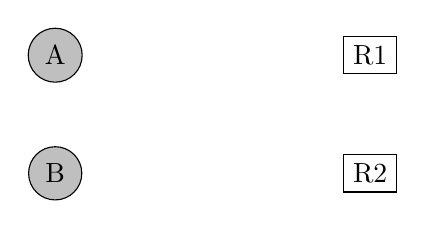
\begin{tikzpicture}
\node[draw,circle,fill=gray!50] (A) at(-2,1.5) {A};
\node[draw,circle,fill=gray!50] (B) at(-2,0) {B};
\node[draw] (R1) at(2,1.5) {R1};
\node[draw] (R2) at(2,0) {R2};
\end{tikzpicture}
\captionof{figure}{Deux processus et deux ressources}
\end{center}
\begin{center}
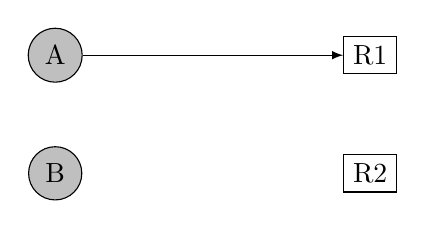
\begin{tikzpicture}
\node[draw,circle,fill=gray!50] (A) at(-2,1.5) {A};
\node[draw,circle,fill=gray!50] (B) at(-2,0) {B};
\node[draw] (R1) at(2,1.5) {R1};
\node[draw] (R2) at(2,0) {R2};
\draw[->,>=latex] (A) to (R1);
\end{tikzpicture}
\captionof{figure}{L'ordonnanceur exécute A.\\A demande R1 qui lui est allouée.}
\end{center}
\begin{center}
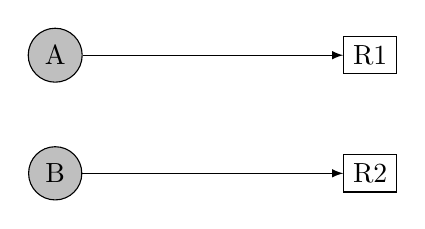
\begin{tikzpicture}
\node[draw,circle,fill=gray!50] (A) at(-2,1.5) {A};
\node[draw,circle,fill=gray!50] (B) at(-2,0) {B};
\node[draw] (R1) at(2,1.5) {R1};
\node[draw] (R2) at(2,0) {R2};
\draw[->,>=latex] (A) to (R1);
\draw[->,>=latex] (B) to (R2);
\end{tikzpicture}
\captionof{figure}{L'ordonnanceur commute.\\B demande R2 qui lui est allouée.}
\end{center}
\begin{center}
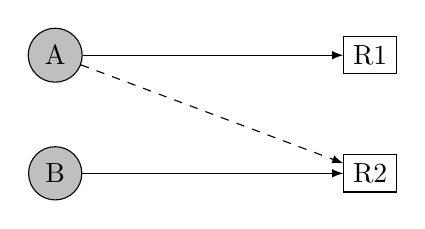
\begin{tikzpicture}
\node[draw,circle,fill=gray!50] (A) at(-2,1.5) {A};
\node[draw,circle,fill=gray!50] (B) at(-2,0) {B};
\node[draw] (R1) at(2,1.5) {R1};
\node[draw] (R2) at(2,0) {R2};
\draw[->,>=latex] (A) to (R1);
\draw[->,>=latex] (B) to (R2);
\draw[->,>=latex, dashed] (A) to (R2);
\end{tikzpicture}
\captionof{figure}{L'ordonnanceur commute.\\A demande R2 qui est déjà allouée. A est bloqué}
\end{center}
\begin{center}
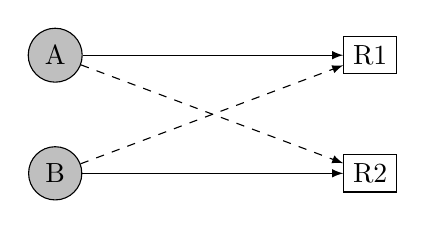
\begin{tikzpicture}
\node[draw,circle,fill=gray!50] (A) at(-2,1.5) {A};
\node[draw,circle,fill=gray!50] (B) at(-2,0) {B};
\node[draw] (R1) at(2,1.5) {R1};
\node[draw] (R2) at(2,0) {R2};
\draw[->,>=latex] (A) to (R1);
\draw[->,>=latex] (B) to (R2);
\draw[->,>=latex, dashed] (A) to (R2);
\draw[->,>=latex, dashed] (B) to (R1);
\end{tikzpicture}
\captionof{figure}{L'ordonnanceur commute.\\B demande R1 qui est déjà allouée. B est bloqué}
\end{center}
Les processus A et B sont en situation d'interblocage.
\subsection{Les conditions de l'interblocage}
L'interblocage est le grand danger de la programmation concurrente. Il existe quatre conditions nécessaires à la présence d'un interblocage, décrites par Edward Grady Coffman en 1971:
\begin{itemize}
\item \textbf{Exclusion mutuelle:} au moins une ressource doit être en accès exclusif.
\item \textbf{Rétention et attente:} un processus détient une ressource et demande une autre ressource détenue par un autre processus.
\item \textbf{Non préemption:} une ressource détenue par un processus ne peut être récupérée de force (\emph{préemptée}) par un autre processus.
\item \textbf{Attente circulaire:} chaque processus attend une ressource détenue par un des autres.
\end{itemize}
\section{Traitement de l'interblocage}
Sans rentrer dans le détail, nous pouvons citer les politiques mises en place pour traiter l'interblocage:
\begin{itemize}
\item \textbf{Politique de guérison:} le système maintient un état permanent des demandes de ressources et résout les éventuels interblocages en tuant un processus.
\item \textbf{Politique de prévention:} le système fait en sorte que les quatre conditions ne soient jamais réunis. Par exemple, ne jamais donner une ressource si elle est déjà utilisée par un autre processus.
\item \textbf{Politique de l'évitement:} à chaque demande de ressource, le système vérifie si cela peut causer un interblocage. Si tel est le cas, l'allocation est retardée.
\item \textbf{Politique de l'autruche:} on ne s'en occupe pas, et on se contente de redémarrer la machine quand trop de processus sont en interblocage. Les trois autres politiques étant très coûteuses cette solution n'est finalement pas si farfelue.
\end{itemize}
\begin{commentprof}
\pagebreak
exemples:
\begin{itemize}
\item accès base de données: deux processus A et B qui demandent des accès exclusifs aux enregistrements d'une base de données. A a verrouillé l'enregistrement R1 et demande l'accès à R2 et réciproquement.
\item problème  Edsger Dijkstra: 5 philosophes en cercle; chacun un plat de spaghettis et une fourchette à gauche. Chaque philosophes a besoin de 2 fourchettes pour manger.
\item circulation de voitures
\begin{center}
\includegraphics[width=8cm]{ressources/circulation.png}
\captionof{figure}{priorité à droite}
\end{center}
\end{itemize}
\end{commentprof}
\end{Form}
\end{document}